\documentclass{standalone}
\usepackage{tikz}
\usetikzlibrary{patterns, positioning}
\usepackage[sfdefault]{ClearSans} %% option 'sfdefault' activates Clear Sans as the default text font
\usepackage[T1]{fontenc}

\begin{document}
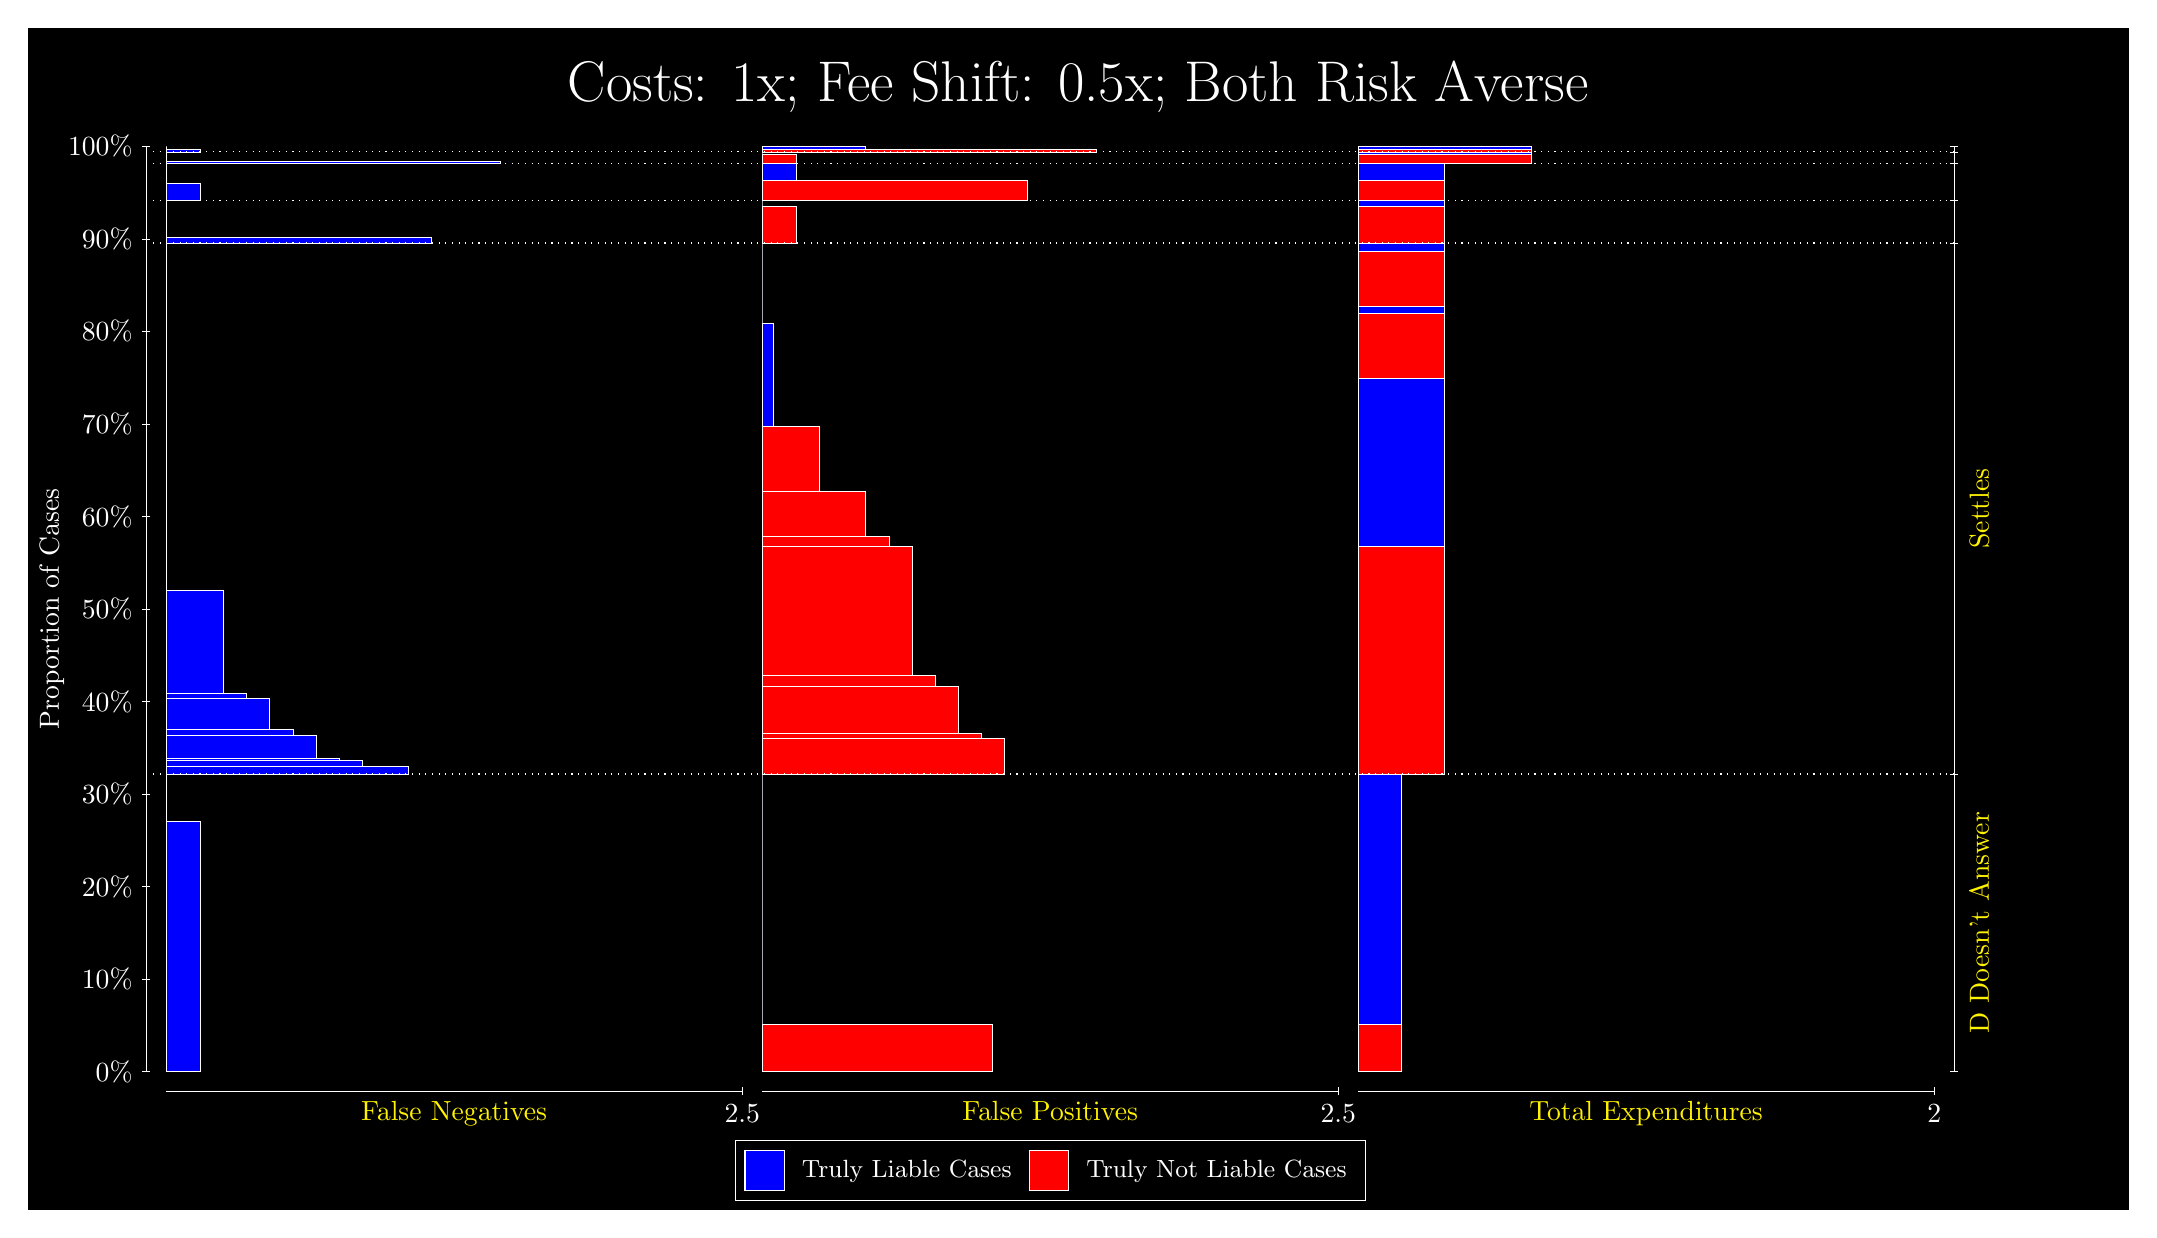
\begin{tikzpicture}
\draw[fill=black] (0,0) rectangle (26.667,15);
\draw[text=white] (0,13.5) rectangle (26.667,15) node[midway] {\huge Costs: 1x; Fee Shift: 0.5x; Both Risk Averse};
\draw[white, very thin] (1.5,1.75) -- (1.5,13.5);
\node[rotate=90, text=white, anchor=center] at (0.3, 7.625) {Proportion of Cases};
\draw[white, very thin] (1.45,1.75) -- (1.55,1.75);
\node[text=white, anchor=east] at (1.45, 1.75) {0\%};
\draw[white, very thin] (1.45,2.925) -- (1.55,2.925);
\node[text=white, anchor=east] at (1.45, 2.925) {10\%};
\draw[white, very thin] (1.45,4.1) -- (1.55,4.1);
\node[text=white, anchor=east] at (1.45, 4.1) {20\%};
\draw[white, very thin] (1.45,5.275) -- (1.55,5.275);
\node[text=white, anchor=east] at (1.45, 5.275) {30\%};
\draw[white, very thin] (1.45,6.45) -- (1.55,6.45);
\node[text=white, anchor=east] at (1.45, 6.45) {40\%};
\draw[white, very thin] (1.45,7.625) -- (1.55,7.625);
\node[text=white, anchor=east] at (1.45, 7.625) {50\%};
\draw[white, very thin] (1.45,8.8) -- (1.55,8.8);
\node[text=white, anchor=east] at (1.45, 8.8) {60\%};
\draw[white, very thin] (1.45,9.975) -- (1.55,9.975);
\node[text=white, anchor=east] at (1.45, 9.975) {70\%};
\draw[white, very thin] (1.45,11.15) -- (1.55,11.15);
\node[text=white, anchor=east] at (1.45, 11.15) {80\%};
\draw[white, very thin] (1.45,12.325) -- (1.55,12.325);
\node[text=white, anchor=east] at (1.45, 12.325) {90\%};
\draw[white, very thin] (1.45,13.5) -- (1.55,13.5);
\node[text=white, anchor=east] at (1.45, 13.5) {100\%};

\draw[white, very thin] (24.457,1.75) -- (24.457,13.5);
\draw[white, very thin] (24.407,1.75) -- (24.507,1.75);
\node[anchor=west] at (24.407, 1.75) {};
\draw[white, very thin] (24.407,5.5283) -- (24.507,5.5283);
\node[anchor=west] at (24.407, 5.5283) {};
\draw[white, very thin] (24.407,12.272) -- (24.507,12.272);
\node[anchor=west] at (24.407, 12.272) {};
\draw[white, very thin] (24.407,12.813) -- (24.507,12.813);
\node[anchor=west] at (24.407, 12.813) {};
\draw[white, very thin] (24.407,13.28) -- (24.507,13.28);
\node[anchor=west] at (24.407, 13.28) {};
\draw[white, very thin] (24.407,13.429) -- (24.507,13.429);
\node[anchor=west] at (24.407, 13.429) {};
\draw[white, very thin] (24.407,13.5) -- (24.507,13.5);
\node[anchor=west] at (24.407, 13.5) {};

\draw[white, very thin, fill=blue] (1.75,1.75) rectangle (2.1891,4.9309);
\draw[white, very thin, fill=red] (1.75,4.9309) rectangle (1.75,5.5283);
\draw[white, very thin, fill=blue] (1.75,5.5283) rectangle (4.8239,5.6204);
\draw[white, very thin, fill=blue] (1.75,5.6204) rectangle (4.2384,5.7015);
\draw[white, very thin, fill=blue] (1.75,5.7015) rectangle (3.9457,5.7227);
\draw[white, very thin, fill=blue] (1.75,5.7227) rectangle (3.6529,6.019);
\draw[white, very thin, fill=blue] (1.75,6.019) rectangle (3.3602,6.0973);
\draw[white, very thin, fill=blue] (1.75,6.0973) rectangle (3.0674,6.495);
\draw[white, very thin, fill=blue] (1.75,6.495) rectangle (2.7746,6.5518);
\draw[white, very thin, fill=blue] (1.75,6.5518) rectangle (2.4819,7.859);
\draw[white, very thin, fill=red] (1.75,7.859) rectangle (1.75,12.272);
\draw[white, very thin, fill=blue] (1.75,12.272) rectangle (5.1167,12.351);
\draw[white, very thin, fill=red] (1.75,12.351) rectangle (1.75,12.813);
\draw[white, very thin, fill=blue] (1.75,12.813) rectangle (2.1891,13.026);
\draw[white, very thin, fill=red] (1.75,13.026) rectangle (1.75,13.28);
\draw[white, very thin, fill=blue] (1.75,13.28) rectangle (5.9949,13.313);
\draw[white, very thin, fill=red] (1.75,13.313) rectangle (1.75,13.429);
\draw[white, very thin, fill=blue] (1.75,13.429) rectangle (2.1891,13.467);
\draw[white, very thin, fill=red] (1.75,13.467) rectangle (1.75,13.5);
\draw[white, very thin, fill=red] (9.3189,1.75) rectangle (12.246,2.3474);
\draw[white, very thin, fill=blue] (9.3189,2.3474) rectangle (9.3189,5.5283);
\draw[white, very thin, fill=red] (9.3189,5.5283) rectangle (12.393,5.9832);
\draw[white, very thin, fill=red] (9.3189,5.9832) rectangle (12.1,6.0446);
\draw[white, very thin, fill=red] (9.3189,6.0446) rectangle (11.807,6.6374);
\draw[white, very thin, fill=red] (9.3189,6.6374) rectangle (11.515,6.7834);
\draw[white, very thin, fill=red] (9.3189,6.7834) rectangle (11.222,8.4151);
\draw[white, very thin, fill=red] (9.3189,8.4151) rectangle (10.929,8.5523);
\draw[white, very thin, fill=red] (9.3189,8.5523) rectangle (10.636,9.1146);
\draw[white, very thin, fill=red] (9.3189,9.1146) rectangle (10.051,9.9417);
\draw[white, very thin, fill=blue] (9.3189,9.9417) rectangle (9.4652,11.249);
\draw[white, very thin, fill=blue] (9.3189,11.249) rectangle (9.3189,12.272);
\draw[white, very thin, fill=red] (9.3189,12.272) rectangle (9.758,12.734);
\draw[white, very thin, fill=blue] (9.3189,12.734) rectangle (9.3189,12.813);
\draw[white, very thin, fill=red] (9.3189,12.813) rectangle (12.686,13.067);
\draw[white, very thin, fill=blue] (9.3189,13.067) rectangle (9.758,13.28);
\draw[white, very thin, fill=red] (9.3189,13.28) rectangle (9.758,13.396);
\draw[white, very thin, fill=blue] (9.3189,13.396) rectangle (9.3189,13.429);
\draw[white, very thin, fill=red] (9.3189,13.429) rectangle (13.564,13.462);
\draw[white, very thin, fill=blue] (9.3189,13.462) rectangle (10.636,13.5);
\draw[white, very thin, fill=red] (16.888,1.75) rectangle (17.437,2.3474);
\draw[white, very thin, fill=blue] (16.888,2.3474) rectangle (17.437,5.5283);
\draw[white, very thin, fill=red] (16.888,5.5283) rectangle (17.986,8.4151);
\draw[white, very thin, fill=blue] (16.888,8.4151) rectangle (17.986,10.551);
\draw[white, very thin, fill=red] (16.888,10.551) rectangle (17.986,11.379);
\draw[white, very thin, fill=blue] (16.888,11.379) rectangle (17.986,11.471);
\draw[white, very thin, fill=red] (16.888,11.471) rectangle (17.986,12.17);
\draw[white, very thin, fill=blue] (16.888,12.17) rectangle (17.986,12.272);
\draw[white, very thin, fill=red] (16.888,12.272) rectangle (17.986,12.734);
\draw[white, very thin, fill=blue] (16.888,12.734) rectangle (17.986,12.813);
\draw[white, very thin, fill=red] (16.888,12.813) rectangle (17.986,13.067);
\draw[white, very thin, fill=blue] (16.888,13.067) rectangle (17.986,13.28);
\draw[white, very thin, fill=red] (16.888,13.28) rectangle (19.083,13.396);
\draw[white, very thin, fill=blue] (16.888,13.396) rectangle (19.083,13.429);
\draw[white, very thin, fill=red] (16.888,13.429) rectangle (19.083,13.462);
\draw[white, very thin, fill=blue] (16.888,13.462) rectangle (19.083,13.5);
\draw[white, dotted] (1.5,5.5283) -- (24.457,5.5283);
\draw[white, dotted] (1.5,12.272) -- (24.457,12.272);
\draw[white, dotted] (1.5,12.813) -- (24.457,12.813);
\draw[white, dotted] (1.5,13.28) -- (24.457,13.28);
\draw[white, dotted] (1.5,13.429) -- (24.457,13.429);
\draw[white, very thin] (1.75,1.5) -- (9.0689,1.5);
\node[text=yellow, anchor=north] at (5.4094, 1.5) {False Negatives};
\draw[white, very thin] (9.0689,1.45) -- (9.0689,1.55);
\node[text=white, anchor=north] at (9.0689, 1.45) {2.5};

\draw[white, very thin] (9.3189,1.5) -- (16.638,1.5);
\node[text=yellow, anchor=north] at (12.978, 1.5) {False Positives};
\draw[white, very thin] (16.638,1.45) -- (16.638,1.55);
\node[text=white, anchor=north] at (16.638, 1.45) {2.5};

\draw[white, very thin] (16.888,1.5) -- (24.207,1.5);
\node[text=yellow, anchor=north] at (20.547, 1.5) {Total Expenditures};
\draw[white, very thin] (24.207,1.45) -- (24.207,1.55);
\node[text=white, anchor=north] at (24.207, 1.45) {2};

\node[text=yellow, centered, rotate=90] at (24.777, 3.6391) {D Doesn't Answer};
\node[text=yellow, centered, rotate=90] at (24.777, 8.9004) {Settles};





\draw (12.978300999999998,1.5) node[draw=none] (baseCoordinate) {};
\begin{scope}[align=center]
        \matrix[scale=0.5, draw=white, below=0.5cm of baseCoordinate, nodes={draw}, column sep=0.1cm]{
            \node[rectangle, draw, minimum width=0.5cm, minimum height=0.5cm, fill=blue] {}; &
            \node[draw=none, font=\small, text=white] (B) {Truly Liable Cases}; &
            \node[rectangle, draw, minimum width=0.5cm, minimum height=0.5cm, fill=red] {}; &
            \node[draw=none, font=\small, text=white] (B) {Truly Not Liable Cases}; \\
            };
\end{scope}

\end{tikzpicture}
\end{document}